\chapteropen
\chapter{Simulating the Universe: A cluster perspective}
\label{app:gal_sim}

\begin{figure}[ht!]
    \centering
    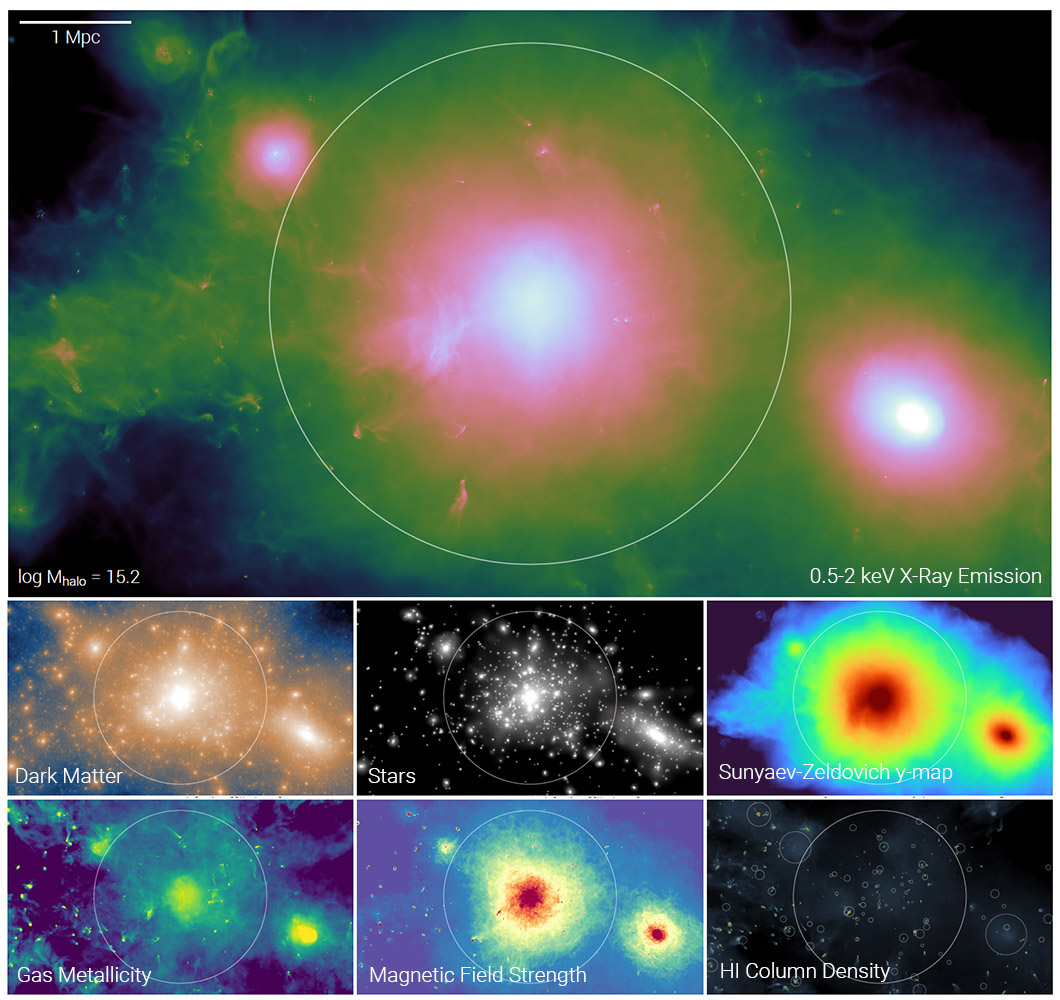
\includegraphics[width=0.90\linewidth]{figures//introduction/TNG-Cluster_halo2_overview.jpg}
    \caption[Massive halo simulation in TNG-Cluster]{Massive halo simulation in TNG-Cluster. Visualizations illustrating the gaseous, stellar, and \gls{dm} distribution and physical properties at $z=0$, with a cluster of total mass $M_{200c}\simeq10^{15.2}\Msun$. Credit: \citep{Nelson_2024}.}
    \label{fig:TNG-cluster-halo}
\end{figure}
In parallel with a full spectrum of electromagnetic observations, cosmological hydrodynamical simulations have become possible with supercomputers since the turn of the century. Examples include the Millennium simulation \citep{Springel_2005}, and more recently, the Illustris project \citep{Vogelsberger_2014} which has spin-offs such as IllustrisTNG (The Next Generation) \citep{Pillepich_2018} and TNG-Cluster \citep{Nelson_2024}, the latter of which focuses on galaxy cluster formation. This is a complex and challenging endeavor as the evolution of the baryonic content of cluster halos includes many facets which need to be considered, including the interplay of gravitational, (magneto)hydrodynamical, radiative, and chemical processes \citep{Donahue_2022}. Inflows of gas from cosmic filaments and feedback driven outflows from \gls{agn} must also be taken into account. Nevertheless, as illustrated in \cref{fig:TNG-cluster-halo}, synthetic imaging in a full range of wavelengths (\eg X-ray, optical, microwave, radio)  is now possible, tracing relevant astrophysical properties of clusters (\eg \gls{icm} distribution, \gls{dm} structure, \gls{cmb} isotropy through \gls{sz} effect). Correlation of the results from these simulations with observed properties of clusters thus allows the refinement of cosmological model parameters. 

For the present thesis, the value of these simulations lies in their ability to connect projected \gls{css} diagnostics to the underlying dynamical histories of cluster galaxies \citep[\eg][]{Ramos-Almendares_2020}. In particular, simulations can test whether galaxies experiencing strong local tidal fields, \gls{bcg} passages, group pre-processing, or repeated high-speed encounters develop the types of signatures identified in this work: deficient \glspl{gcs}, asymmetric \gls{gc} distributions, altered blue-\gls{gc} fractions, and enhanced \gls{icgc} density. A future simulation framework which explicitly tracks blue and red \gls{gc} subpopulations, stellar halos, \gls{icl}, gas, and \gls{dm} would therefore provide a direct way to interpret the observational diagnostics developed in this thesis.

One limitation is that individual \glspl{gc} are generally not resolved directly in large cosmological volumes. Connecting simulations to the \gls{css} diagnostics used in this thesis would therefore require either particle-tagging methods, semi-analytic prescriptions for \gls{gc} formation and disruption, or high-resolution zoom simulations capable of following compact stellar populations more explicitly.
